\appendix
\chapter[Transitional RBP flows]{Transitional Rayleigh-B\'{e}nard Poiseuille flows}\label{app:rbp}
In Appendix \ref{app:rbp}, we provide additional results and discussion pertaining to our investigation in transitional Rayleigh-B\'{e}nard Poiseuille flows in \S \ref{chap:3}. The mathematical notations and definitions follow those defined in \S \ref{chap:3}.
\section{Simulation parameters for $Ra$-$Re$ sweep}\label{app:params}
\begin{table}\scriptsize
\centering
\begin{tabular}{l l l l l l l l}
    Ra & Re & $N_z$ & $dt$ & $T$ & $\frac{d}{\kappa}$\\
    \hline
    \hline
    0	&	1050	&	64	&	0.1	&	8000	&	-    \\
    0	&	2000	&	128	&	0.02	&	3000	&	- \\
    \hline
    2000	&	0	&	64	&	0.05	&	50	&	25       \\
    2000	&	0.1	&	64	&	0.005	&	5	&	25       \\
    2000	&	1	&   64	&	0.01	&	50	&	25       \\
    2000	&	10	&	64	&	0.05	&	50	&	2.5      \\
    2000	&	100	&	64	&	0.1	&	50	&	0.25         \\
    2000	&	500	&	64	&	0.1	&	50	&	0.05         \\
    2000	&	750	&	64	&	0.1	&	50	&	0.033        \\
    2000	&	1000&	64	&	0.1	&	50	&	0.025    \\
    2000	&	1050&	64	&	0.1	&	8000	&	3.81    \\
    2000	&	2000&	128	&	0.02	&	2800	&	0.75 \\
    \hline
    3000	&	0	&	64	&	0.05	&	3000	&	1500     \\
    3000	&	0.1	&	64	&	0.005	&	300	&	1500         \\
    3000	&	1	&	64	&	0.05	&	100	&	50           \\
    3000	&	10	&	64	&	0.05	&	50	&	2.5          \\
    3000	&	100	&	64	&	0.1	&	10000	&	50           \\
    3000	&	500	&	64	&	0.1	&	50	&	0.05             \\
    3000	&	750	&	64	&	0.1	&	50	&	0.033            \\
    3000	&	1000&	64	&	0.1	&	50	&	0.025        \\
    3000	&	1050&	64	&	0.1	&	8000	&	3.81         \\
    3000	&	2000&	128	&	0.02	&	2800	&	0.75 \\
    \hline
    5000	&	0	&	64	&	0.005	&	1200	&	600      \\
    5000	&	0.1	&	64	&	0.001	&	800	&	4000         \\
    5000	&	1	&	64	&	0.01	&	2500	&	1250     \\
    5000	&	10	&	64	&	0.05	&	500	&	25           \\
    5000	&	100	&	64	&	0.1	&	1000	&	5            \\
    5000	&	500	&	64	&	0.05	&	8000	&	8       \\
    5000	&	750	&	64	&	0.05	&	8000	&	5.33     \\
    5000	&	1000&	64	&	0.02	&	8000	&	4    \\
    5000	&	1050&	64	&	0.02	&	8000	&	3.81     \\
    5000	&	2000&	128	&	0.02	&	2800	&	0.75 \\ 
    \hline
    8000	&	0	&	64	&	0.0025	&	600	&	300          \\
    8000	&	0.1	&	64	&	0.0005	&	600	&	3000         \\
    8000	&	1	&	64	&	0.005	&	600	&	300          \\
    8000	&	10	&	64	&	0.05	&	500	&	25           \\
    8000	&	100	&	64	&	0.1	&	5000	&	25           \\
    8000	&	500	&	64	&	0.05	&	10000	&	10       \\
    8000	&	750	&	64	&	0.05	&	8000	&	5.33     \\
    8000	&	1000&	64	&	0.02	&	8000	&	4    \\
    8000	&	1050&	64	&	0.02	&	8000	& 3.81   \\
    8000	&	2000&	128	&	0.02	&	2800	&	0.75 \\
    \hline
    10000	&	0	&	64	&	0.0025	&	1000	&	500      \\
    10000	&	0.1	&	64	&	0.00025	&	800	&	4000         \\
    10000	&	1	&	64	&	0.0025	&	600	&	300          \\
    10000	&	10	&	64	&	0.05	&	12000	&	600      \\
    10000	&	100	&	64	&	0.1	&	8000	&	40           \\
    10000	&	500	&	64	&	0.05	&	8000	&	8        \\
    10000	&	750	&	64	&	0.05	&	8000	&	5.33     \\
    10000	&	1000	&	64	&	0.02	&	8000	&	4    \\
    10000	&	1050	&	64	&	0.02	&	8000	& 3.81   \\
    10000	&	2000	&	128	&	0.02	&	2800	&	0.75 \\
\end{tabular}
\caption{The summary of the spatial and temporal resolution for a given $Re$, $Ra$. $N_z$ denotes the number of Fourier expansions in the $z$-direction. $dt, T, d/\kappa$ denotes the timestep, final time and the final time scaled by the thermal timescale.}
\label{tab:simulations}
\end{table}
The spectral/\emph{hp} quadrilateral element width, heights and polynomial order are kept constant for all simulations, $(\Delta x, \Delta y|_{y=\pm h}, \Delta y|_{y=0}, P) = (0.1\pi,0.0549,0.367,4)$.
To resolve the high gradients near the wall, the quadrilateral element heights are bunched near the wall, $\Delta y|_{y=\pm h}$, and expanded in the channel center, $\Delta y|_{y=0}$.
The basis type employed here consists of the modified Jacobi polynomials, known as the \emph{modified} basis (see \S \ref{sec:nm_modalexpansions}).
Table \ref{tab:simulations} describes the number of Fourier expansions, $N_z$, and temporal resolution of 52 numerical experiments at $Re = 0, 0.1, 1, 10, 100, 500, 750, 1000, 1050$, $2000$, and $Ra = 0, 2000, 3000, 5000, 8000, 10000$ with $Pr = 1$ and a large aspect ratio, $\Gamma = 4\pi$. 
The initial conditions of all numerical experiments were sampled from a statistically stationary solution based on the time history of the Nusselt number and shear.
The laminar solution obtained for  $Ra = 0$ , $Re \leq 1000$ has been omitted in table \ref{tab:simulations}.

\section{Buoyancy-driven regime}\label{app:buoyancy}
\begin{figure}
    \centering
    \includegraphics[width=\linewidth]{TransitionalRBP/Figures/PhaseSpace/BuoyancyStatistics.pdf}
    \caption{The wall-normal distribution of temporal and plane- averaged (a) streamwise velocity, (b) temperature, (c) fluctuating wall-normal velocity squared normalised by thermal velocity scale, (d) fluctuating temperature squared and (e) fluctuating span- and streamwise velocities squared normalised by thermal velocity scale of buoyancy-driven regime shaded in red in figure \ref{fig:rarephase}.}
    \label{fig:BuoyancyStatistics}
\end{figure}

We present the first- and second-order statistics of the buoyancy-dominated regime (shaded in red), consisting of the (1) SDC \& ISRs, and (2) ISRs states in figure \ref{fig:BuoyancyStatistics}, illustrating its temporal and plane-averaged streamwise velocity, $\langle w \rangle_{x,z,t}$, temperature, $\langle \theta \rangle_{x,z,t}$, fluctuating wall-normal velocity squared normalised by thermal velocity scale, $\langle \tilde{v} \tilde{v} \rangle_{x,z,t}/u_\kappa^2$, fluctuating temperature squared, $\langle \tilde{\theta}\tilde{\theta} \rangle_{x,z,t}$ and fluctuating span- and streamwise velocities squared normalised by thermal velocity scale, $\langle \tilde{u}\tilde{u} + \tilde{w}\tilde{w} \rangle_{x,z,t}/u_\kappa^2$.
We note that the fluctuating components are defined about a temporal-planar averaged quantity, i.e $\tilde{\mathbf{u}} = \mathbf{u} - \langle \mathbf{u} \rangle_{x,z,t}$.
The mean temperature profiles (figure \ref{fig:BuoyancyStatistics}(b)), and the fluctuating span- and streamwise velocities (figure \ref{fig:BuoyancyStatistics}(f)) are visually similar for the same $Ra$, and are nearly independent of $Re$.
However, we observe the dependence on $Re$ at $Ra = 3000$ in the fluctuating temperature squared (figure \ref{fig:BuoyancyStatistics}(d)), and fluctuating wall-normal velocities (figure \ref{fig:BuoyancyStatistics}(c)), likely due to variations in convection structures, particularly in the convection roll wavenumbers. 
A detailed analysis of how the statistical properties vary with roll wavenumber is beyond the scope of this work.
We propose that the underlying flow structure, consisting of convection rolls, describes the buoyancy-driven regime, shaded in red in figure \ref{fig:rarephase}.
In this regime, the strength of the convection is primarily controlled by $Ra$, akin to RBC, and remains independent of $Re$.

\section{Shear-driven regime}\label{app:shear}
\begin{figure}
    \centering
    \includegraphics[width=\linewidth]{TransitionalRBP/Figures/PhaseSpace/ShearStatistics.pdf}
    \caption{The wall-normal distribution of temporal and plane- averaged (a) streamwise velocity, (b) temperature, (c) fluctuating streamwise velocity squared, (d) fluctuating wall-normal velocity squared, (e) fluctuating spanwise velocities squared,  (f) fluctuating Reynolds stresses and (g) fluctuating temperature squared in the shear-driven regime shaded in blue in figure \ref{fig:rarephase}.}
    \label{fig:sheardrivenstatistics}
\end{figure}

As $Re$ falls within the range of $1050 \leq Re \leq 2000$, shear-driven turbulence dominates, where the impact of $Ra$ on the first- and second-order statistics is weakly dependent on $Ra$ in figure \ref{fig:sheardrivenstatistics}.
Figure \ref{fig:sheardrivenstatistics} describes the temporal and plane-averaged streamwise velocity, $\langle w \rangle_{x,z,t}$, temperature, $\langle \theta \rangle_{x,z,t}$, fluctuating streamwise velocity squared, $\langle \tilde{w}\tilde{w} \rangle_{x,z,t}$, fluctuating wall-normal velocity squared, $\langle \tilde{v} \tilde{v} \rangle_{x,z,t}$, fluctuating spanwise velocities squared, $\langle \tilde{u}\tilde{u} \rangle_{x,z,t}$, fluctuating Reynolds stresses $\langle \tilde{v}\tilde{w} \rangle_{x,z,t}$, and fluctuating temperature squared, $\langle \tilde{\theta}\tilde{\theta} \rangle_{x,z,t}$ at $Re = 2000, 1050$ for $Ra \in [0, 10000]$.
The flow structures appear as uniform, featureless turbulence \citep{tuckerman_turbulent-laminar_2014} at $Re = 2000$, independent of $Ra$.
\begin{figure}
    \centering
    \includegraphics[width=\linewidth]{TransitionalRBP/Figures/Appendix/Re2000-BotSpaceTimeCompiled.pdf}
    \caption{Spacetime plots of near-wall, wall-normal and spanwise perturbation kinetic energy for $Re = 2000$, $t\in[0, 2800]$, $\Gamma= 4\pi$ at (a) $Ra = 10000$, (b) $Ra = 8000$, (c) $Ra = 5000$, (d) $Ra = 3000$, (e) $Ra = 2000$, (f) $Ra = 0$.}
    \label{fig:spacetime-Re2000}
\end{figure}
The spacetime figure of near-wall ($y^+ = 15$), wall-normal and spanwise perturbation kinetic energy, $\mathcal{E}_{u'+v'}$, at $Re = 2000$, $t \in [0,2800]$, illustrating spatially uniform featureless turbulence, visually distinguishable withn $Ra \in [0, 10000]$, corroborating with their $Ra$-independent first- and second-order statistics in figure \ref{fig:sheardrivenstatistics}.
In other words, the dominant physical mechanism is shear-driven turbulence at $Re = 2000$, independent of $Ra$.

As $Re$ approaches $Re = 1050$, the midplane temperature in figure \ref{fig:rarephase} shows regions of spatially localised structures, indicating the presence of turbulent-laminar bands, described in figure \ref{fig:spacetime-Ra0k-Re1.05k} and \ref{fig:spacetime-Ra10k-Re1.05k} later.
The mean streamwise velocity and temperature gradients at both ends of the wall, and second-order statistics, are enhanced slightly from $Ra = 0$ to $Ra = 10000$.
This enhancement could be due to the coexistence of longitudinal rolls with turbulent bands at $Ra = 10000$, discussed in \S \ref{sec:rbp_3.3}.
Notably, we have also included the statistics for a subcritical case ($Ra < Ra_{\parallel}$) at $Ra = 1000$, indicating the presence of subcritical effects as the statistics are slightly enhanced from $Ra = 0$ to $Ra = 1000$, reported by \citet{john_soundar_jerome_transient_2012}.
Nonetheless, there is a distinct change of state between $Re = 1000$ to $1050$ (see figure \ref{fig:rarephase}), marked by the transition from the longitudinal/intermittent roll regime to shear-driven turbulence at $Re \geq 1050$, thus, shaded in blue in figure \ref{fig:rarephase}.

\section{Growth rates of primary instabilities}\label{app:long-pri}
\begin{figure}
    \centering
    \includegraphics[width=\linewidth]{TransitionalRBP/Figures/Appendix/peigs.pdf}
    \caption{Growth rates of primary instabilities at $Ra = 10000, 8000, 5000, 3000, 2000$ leading to the onset of longitudinal rolls against spanwise wavenumber of $\alpha d$ at $Re = 1050$.}
    \label{fig:long-pri-instab}
\end{figure}

Figure \ref{fig:long-pri-instab} shows the eigenvalues of the primary instabilities as a function of its spanwise wavenumber $\alpha d$, leading to the onset of longitudinal rolls at $Re = 1050$. The results are obtained using a Chebyshev-collocation method discretised by 51 Chebyshev polynomials \citep{driscoll_chebfun_2014}. The crosses denote the spanwise wavenumbers admissible within the domain $\Gamma = \pi/2$, where $\alpha d = 4$ corresponds to the dominant eigenmode.

\chapter[State-space structure of SDC]{State-space structure of spiral defect chaos}\label{app:sdc}
In Appendix \ref{app:sdc}, we provide additional results and discussion pertaining to our investigation in the state-space structure of spiral defect chaos in Rayleigh-B\'{e}nard convection in \S \ref{chap:4}. The mathematical notations and definitions follow those defined in \S \ref{chap:4}.
\section{Verification of linear stability analysis}\label{app:sdc_appA}
\begin{figure}
    \centering
    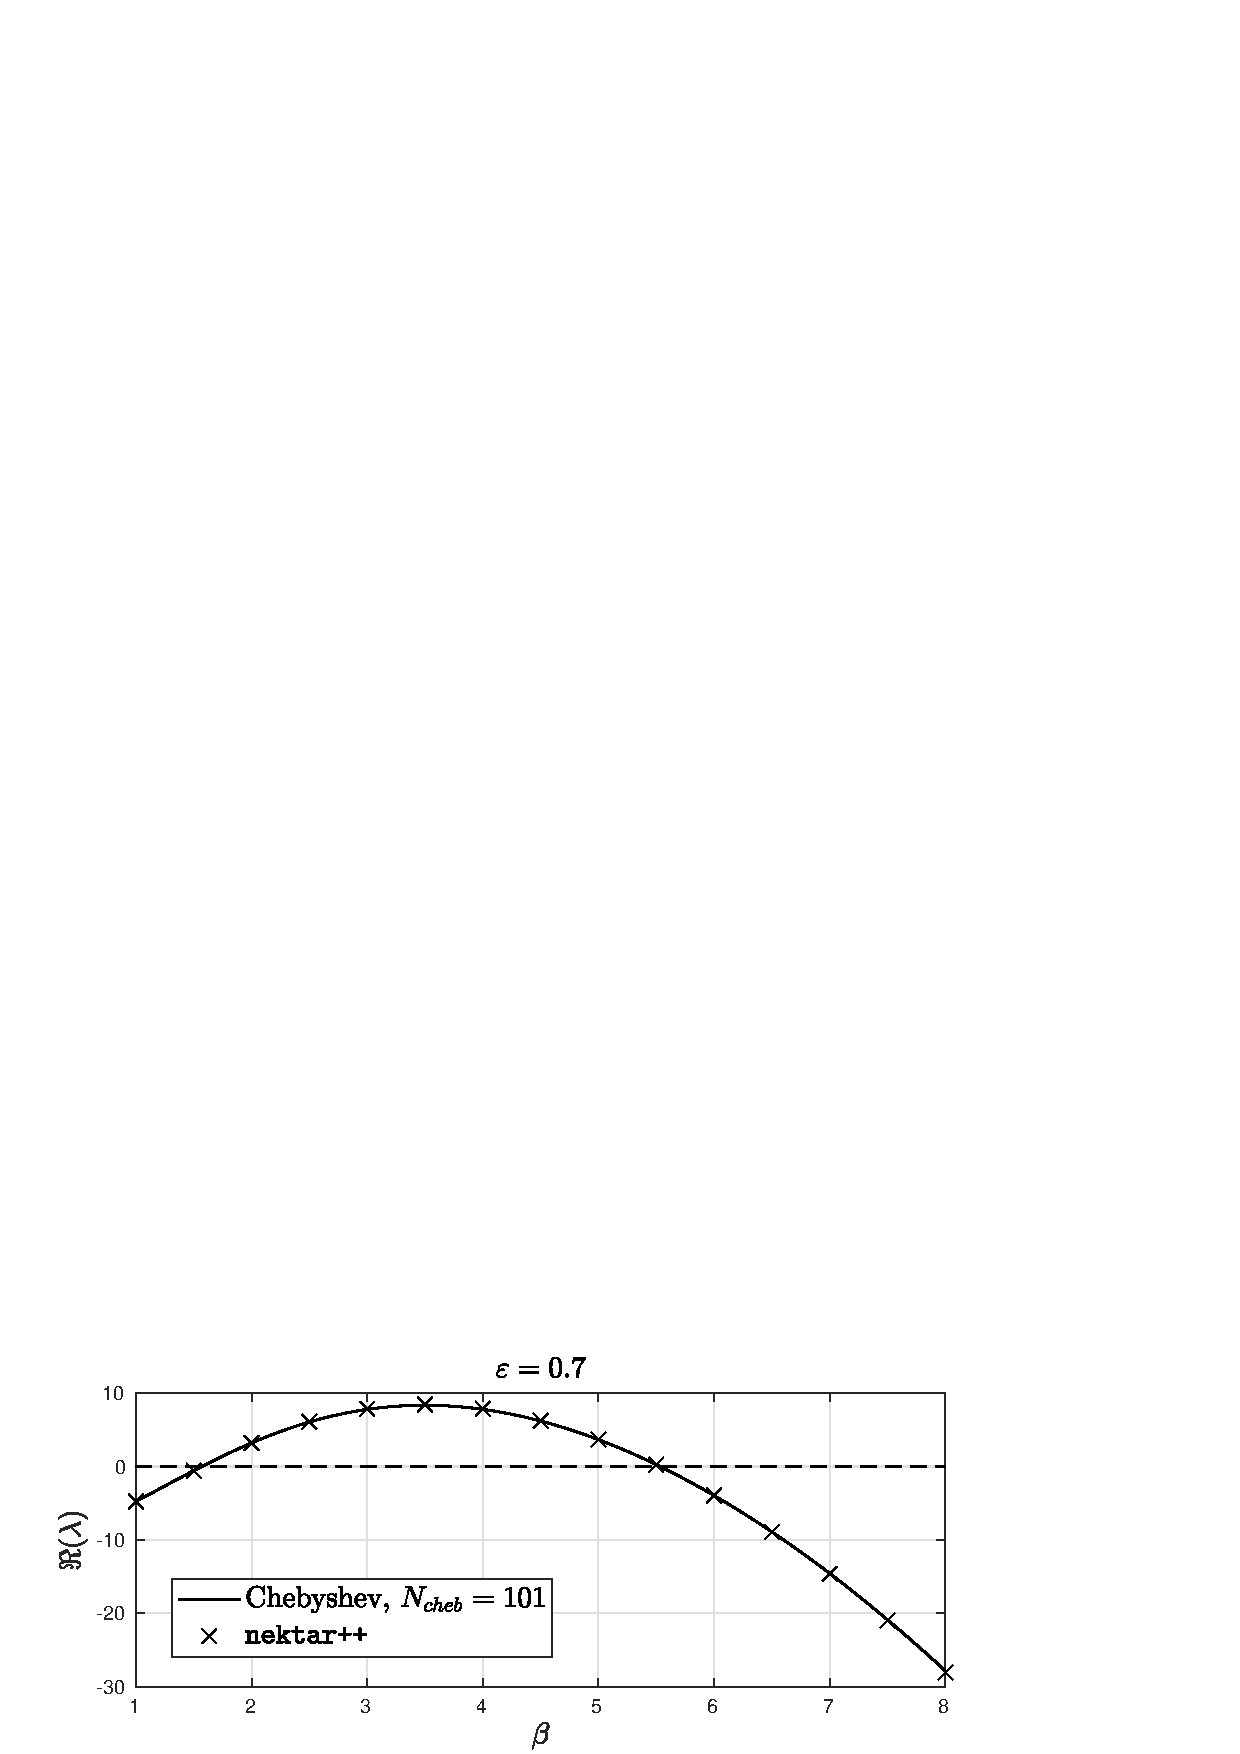
\includegraphics[width=1\textwidth]{StateSpaceStructureOfSDC/Figures/evComparisonPlot.pdf}
    \caption{Eigenvalues of primary instabilities of RBC at $\varepsilon = 0.7$ computed in Nektar++ compared against a Chebyshev-collocation method with $101$ Chebyshev expansions.}
    \label{fig:evvalidation}
\end{figure}

Figure \ref{fig:evvalidation} shows the eigenvalues as a function of spanwise wavenumber $\beta$ of RBC at $\varepsilon = 0.7$. The results are obtained using Nektar++ and compared against a Chebyshev-collocation method discretised by 101 Chebyshev polynomials \citep{driscoll_chebfun_2014}.

\section{Additional elementary states and ISRs}\label{app:sdc_appB}
Figure \ref{fig:10elementaries} presents snapshots of temperature slices ($\theta(x,z)|_{d/2}$), depicting ten distinct elementary states. These states are obtained within a minimal domain $\Gamma = 4\pi$, consisting of eight stationary states (figures \ref{fig:10elementaries}(a-h)) and two travelling-wave states (figures \ref{fig:10elementaries}(i,j)).
Figure \ref{fig:ISRs} features a snapshot of fourteen ideal straight rolls (ISRs), and they satisfy rotational symmetry about the $y$-axis and mirror symmetries about the $x$- and $z$-axes due to the horizontal isotropy of the present system. These ISRs represent stable fixed-points in the state space of figures \ref{fig:statespace-sdc-isr-transient}, \ref{fig:statespace-sdc-isr-elems}, \ref{fig:statespace-sdc-isr-elems-edge}, \ref{fig:phasespacetraj}.

\begin{figure}
    \centering
    \includegraphics[width=\textwidth]{StateSpaceStructureOfSDC/Figures/elementaries.pdf}
    \caption{Temperature snapshots, $\theta(x,z)|_{y=d/2}$, of 10 elementary states confined within a minimal domain $\Gamma = 4\pi$: (a) steady `forked-A' state, (b) steady `forked-B' state, (c) steady `forked-c' state, (d) steady `twin-armed' state, (e) steady `tri-rolls' state, (f) travelling-wave `O-a' state, (g) travelling-wave `O-b' state, (h) steady `keyhole' state, (i) relative periodic orbit `eye' state, (j) relative periodic orbit `S' state. We note that these states are distinct and are not equivalent to each other under any combination of spatial rotations, translations or reflections. Although elementary states (a-c) and (f-g) appear visually to be equivalent under certain symmetries, they are in fact distinct, evidenced by their differing $L_2$-norms in figure \ref{fig:statespace-sdc-isr-elems}.}
    \label{fig:10elementaries}
\end{figure}

\begin{figure}
    \centering
    \includegraphics[width=\textwidth]{StateSpaceStructureOfSDC/Figures/ISRs.pdf}
    \caption{Temperature snapshots, $\theta(x,z)|_{y=d/2}$, of 14 stable ideal straight rolls (ISRs) confined within a minimal domain, $\Gamma = 4\pi$. Plots (a-n) are ordered in increasing wavenumbers, $q \in (2/d, 3.35/d)$. We note that these states are distinct and are not equivalent to each other under any combinations of spatial rotation, translation or reflection.}
    \label{fig:ISRs}
\end{figure}
